
% Default to the notebook output style

    


% Inherit from the specified cell style.




    
\documentclass[11pt]{article}

    
    
    \usepackage[T1]{fontenc}
    % Nicer default font (+ math font) than Computer Modern for most use cases
    \usepackage{mathpazo}

    % Basic figure setup, for now with no caption control since it's done
    % automatically by Pandoc (which extracts ![](path) syntax from Markdown).
    \usepackage{graphicx}
    % We will generate all images so they have a width \maxwidth. This means
    % that they will get their normal width if they fit onto the page, but
    % are scaled down if they would overflow the margins.
    \makeatletter
    \def\maxwidth{\ifdim\Gin@nat@width>\linewidth\linewidth
    \else\Gin@nat@width\fi}
    \makeatother
    \let\Oldincludegraphics\includegraphics
    % Set max figure width to be 80% of text width, for now hardcoded.
    \renewcommand{\includegraphics}[1]{\Oldincludegraphics[width=.8\maxwidth]{#1}}
    % Ensure that by default, figures have no caption (until we provide a
    % proper Figure object with a Caption API and a way to capture that
    % in the conversion process - todo).
    \usepackage{caption}
    \DeclareCaptionLabelFormat{nolabel}{}
    \captionsetup{labelformat=nolabel}

    \usepackage{adjustbox} % Used to constrain images to a maximum size 
    \usepackage{xcolor} % Allow colors to be defined
    \usepackage{enumerate} % Needed for markdown enumerations to work
    \usepackage{geometry} % Used to adjust the document margins
    \usepackage{amsmath} % Equations
    \usepackage{amssymb} % Equations
    \usepackage{textcomp} % defines textquotesingle
    % Hack from http://tex.stackexchange.com/a/47451/13684:
    \AtBeginDocument{%
        \def\PYZsq{\textquotesingle}% Upright quotes in Pygmentized code
    }
    \usepackage{upquote} % Upright quotes for verbatim code
    \usepackage{eurosym} % defines \euro
    \usepackage[mathletters]{ucs} % Extended unicode (utf-8) support
    \usepackage[utf8x]{inputenc} % Allow utf-8 characters in the tex document
    \usepackage{fancyvrb} % verbatim replacement that allows latex
    \usepackage{grffile} % extends the file name processing of package graphics 
                         % to support a larger range 
    % The hyperref package gives us a pdf with properly built
    % internal navigation ('pdf bookmarks' for the table of contents,
    % internal cross-reference links, web links for URLs, etc.)
    \usepackage{hyperref}
    \usepackage{longtable} % longtable support required by pandoc >1.10
    \usepackage{booktabs}  % table support for pandoc > 1.12.2
    \usepackage[inline]{enumitem} % IRkernel/repr support (it uses the enumerate* environment)
    \usepackage[normalem]{ulem} % ulem is needed to support strikethroughs (\sout)
                                % normalem makes italics be italics, not underlines
    \usepackage{mathrsfs}
    

    
    
    % Colors for the hyperref package
    \definecolor{urlcolor}{rgb}{0,.145,.698}
    \definecolor{linkcolor}{rgb}{.71,0.21,0.01}
    \definecolor{citecolor}{rgb}{.12,.54,.11}

    % ANSI colors
    \definecolor{ansi-black}{HTML}{3E424D}
    \definecolor{ansi-black-intense}{HTML}{282C36}
    \definecolor{ansi-red}{HTML}{E75C58}
    \definecolor{ansi-red-intense}{HTML}{B22B31}
    \definecolor{ansi-green}{HTML}{00A250}
    \definecolor{ansi-green-intense}{HTML}{007427}
    \definecolor{ansi-yellow}{HTML}{DDB62B}
    \definecolor{ansi-yellow-intense}{HTML}{B27D12}
    \definecolor{ansi-blue}{HTML}{208FFB}
    \definecolor{ansi-blue-intense}{HTML}{0065CA}
    \definecolor{ansi-magenta}{HTML}{D160C4}
    \definecolor{ansi-magenta-intense}{HTML}{A03196}
    \definecolor{ansi-cyan}{HTML}{60C6C8}
    \definecolor{ansi-cyan-intense}{HTML}{258F8F}
    \definecolor{ansi-white}{HTML}{C5C1B4}
    \definecolor{ansi-white-intense}{HTML}{A1A6B2}
    \definecolor{ansi-default-inverse-fg}{HTML}{FFFFFF}
    \definecolor{ansi-default-inverse-bg}{HTML}{000000}

    % commands and environments needed by pandoc snippets
    % extracted from the output of `pandoc -s`
    \providecommand{\tightlist}{%
      \setlength{\itemsep}{0pt}\setlength{\parskip}{0pt}}
    \DefineVerbatimEnvironment{Highlighting}{Verbatim}{commandchars=\\\{\}}
    % Add ',fontsize=\small' for more characters per line
    \newenvironment{Shaded}{}{}
    \newcommand{\KeywordTok}[1]{\textcolor[rgb]{0.00,0.44,0.13}{\textbf{{#1}}}}
    \newcommand{\DataTypeTok}[1]{\textcolor[rgb]{0.56,0.13,0.00}{{#1}}}
    \newcommand{\DecValTok}[1]{\textcolor[rgb]{0.25,0.63,0.44}{{#1}}}
    \newcommand{\BaseNTok}[1]{\textcolor[rgb]{0.25,0.63,0.44}{{#1}}}
    \newcommand{\FloatTok}[1]{\textcolor[rgb]{0.25,0.63,0.44}{{#1}}}
    \newcommand{\CharTok}[1]{\textcolor[rgb]{0.25,0.44,0.63}{{#1}}}
    \newcommand{\StringTok}[1]{\textcolor[rgb]{0.25,0.44,0.63}{{#1}}}
    \newcommand{\CommentTok}[1]{\textcolor[rgb]{0.38,0.63,0.69}{\textit{{#1}}}}
    \newcommand{\OtherTok}[1]{\textcolor[rgb]{0.00,0.44,0.13}{{#1}}}
    \newcommand{\AlertTok}[1]{\textcolor[rgb]{1.00,0.00,0.00}{\textbf{{#1}}}}
    \newcommand{\FunctionTok}[1]{\textcolor[rgb]{0.02,0.16,0.49}{{#1}}}
    \newcommand{\RegionMarkerTok}[1]{{#1}}
    \newcommand{\ErrorTok}[1]{\textcolor[rgb]{1.00,0.00,0.00}{\textbf{{#1}}}}
    \newcommand{\NormalTok}[1]{{#1}}
    
    % Additional commands for more recent versions of Pandoc
    \newcommand{\ConstantTok}[1]{\textcolor[rgb]{0.53,0.00,0.00}{{#1}}}
    \newcommand{\SpecialCharTok}[1]{\textcolor[rgb]{0.25,0.44,0.63}{{#1}}}
    \newcommand{\VerbatimStringTok}[1]{\textcolor[rgb]{0.25,0.44,0.63}{{#1}}}
    \newcommand{\SpecialStringTok}[1]{\textcolor[rgb]{0.73,0.40,0.53}{{#1}}}
    \newcommand{\ImportTok}[1]{{#1}}
    \newcommand{\DocumentationTok}[1]{\textcolor[rgb]{0.73,0.13,0.13}{\textit{{#1}}}}
    \newcommand{\AnnotationTok}[1]{\textcolor[rgb]{0.38,0.63,0.69}{\textbf{\textit{{#1}}}}}
    \newcommand{\CommentVarTok}[1]{\textcolor[rgb]{0.38,0.63,0.69}{\textbf{\textit{{#1}}}}}
    \newcommand{\VariableTok}[1]{\textcolor[rgb]{0.10,0.09,0.49}{{#1}}}
    \newcommand{\ControlFlowTok}[1]{\textcolor[rgb]{0.00,0.44,0.13}{\textbf{{#1}}}}
    \newcommand{\OperatorTok}[1]{\textcolor[rgb]{0.40,0.40,0.40}{{#1}}}
    \newcommand{\BuiltInTok}[1]{{#1}}
    \newcommand{\ExtensionTok}[1]{{#1}}
    \newcommand{\PreprocessorTok}[1]{\textcolor[rgb]{0.74,0.48,0.00}{{#1}}}
    \newcommand{\AttributeTok}[1]{\textcolor[rgb]{0.49,0.56,0.16}{{#1}}}
    \newcommand{\InformationTok}[1]{\textcolor[rgb]{0.38,0.63,0.69}{\textbf{\textit{{#1}}}}}
    \newcommand{\WarningTok}[1]{\textcolor[rgb]{0.38,0.63,0.69}{\textbf{\textit{{#1}}}}}
    
    
    % Define a nice break command that doesn't care if a line doesn't already
    % exist.
    \def\br{\hspace*{\fill} \\* }
    % Math Jax compatibility definitions
    \def\gt{>}
    \def\lt{<}
    \let\Oldtex\TeX
    \let\Oldlatex\LaTeX
    \renewcommand{\TeX}{\textrm{\Oldtex}}
    \renewcommand{\LaTeX}{\textrm{\Oldlatex}}
    % Document parameters
    % Document title
    \title{Bootstrapping - Practical Lesson 6}
    \author{Matteo Sani \\ \href{mailto:matteosan1@gmail.com}{matteosan1@gmail.com}}
      
    
    

    % Pygments definitions
    
\makeatletter
\def\PY@reset{\let\PY@it=\relax \let\PY@bf=\relax%
    \let\PY@ul=\relax \let\PY@tc=\relax%
    \let\PY@bc=\relax \let\PY@ff=\relax}
\def\PY@tok#1{\csname PY@tok@#1\endcsname}
\def\PY@toks#1+{\ifx\relax#1\empty\else%
    \PY@tok{#1}\expandafter\PY@toks\fi}
\def\PY@do#1{\PY@bc{\PY@tc{\PY@ul{%
    \PY@it{\PY@bf{\PY@ff{#1}}}}}}}
\def\PY#1#2{\PY@reset\PY@toks#1+\relax+\PY@do{#2}}

\expandafter\def\csname PY@tok@w\endcsname{\def\PY@tc##1{\textcolor[rgb]{0.73,0.73,0.73}{##1}}}
\expandafter\def\csname PY@tok@c\endcsname{\let\PY@it=\textit\def\PY@tc##1{\textcolor[rgb]{0.25,0.50,0.50}{##1}}}
\expandafter\def\csname PY@tok@cp\endcsname{\def\PY@tc##1{\textcolor[rgb]{0.74,0.48,0.00}{##1}}}
\expandafter\def\csname PY@tok@k\endcsname{\let\PY@bf=\textbf\def\PY@tc##1{\textcolor[rgb]{0.00,0.50,0.00}{##1}}}
\expandafter\def\csname PY@tok@kp\endcsname{\def\PY@tc##1{\textcolor[rgb]{0.00,0.50,0.00}{##1}}}
\expandafter\def\csname PY@tok@kt\endcsname{\def\PY@tc##1{\textcolor[rgb]{0.69,0.00,0.25}{##1}}}
\expandafter\def\csname PY@tok@o\endcsname{\def\PY@tc##1{\textcolor[rgb]{0.40,0.40,0.40}{##1}}}
\expandafter\def\csname PY@tok@ow\endcsname{\let\PY@bf=\textbf\def\PY@tc##1{\textcolor[rgb]{0.67,0.13,1.00}{##1}}}
\expandafter\def\csname PY@tok@nb\endcsname{\def\PY@tc##1{\textcolor[rgb]{0.00,0.50,0.00}{##1}}}
\expandafter\def\csname PY@tok@nf\endcsname{\def\PY@tc##1{\textcolor[rgb]{0.00,0.00,1.00}{##1}}}
\expandafter\def\csname PY@tok@nc\endcsname{\let\PY@bf=\textbf\def\PY@tc##1{\textcolor[rgb]{0.00,0.00,1.00}{##1}}}
\expandafter\def\csname PY@tok@nn\endcsname{\let\PY@bf=\textbf\def\PY@tc##1{\textcolor[rgb]{0.00,0.00,1.00}{##1}}}
\expandafter\def\csname PY@tok@ne\endcsname{\let\PY@bf=\textbf\def\PY@tc##1{\textcolor[rgb]{0.82,0.25,0.23}{##1}}}
\expandafter\def\csname PY@tok@nv\endcsname{\def\PY@tc##1{\textcolor[rgb]{0.10,0.09,0.49}{##1}}}
\expandafter\def\csname PY@tok@no\endcsname{\def\PY@tc##1{\textcolor[rgb]{0.53,0.00,0.00}{##1}}}
\expandafter\def\csname PY@tok@nl\endcsname{\def\PY@tc##1{\textcolor[rgb]{0.63,0.63,0.00}{##1}}}
\expandafter\def\csname PY@tok@ni\endcsname{\let\PY@bf=\textbf\def\PY@tc##1{\textcolor[rgb]{0.60,0.60,0.60}{##1}}}
\expandafter\def\csname PY@tok@na\endcsname{\def\PY@tc##1{\textcolor[rgb]{0.49,0.56,0.16}{##1}}}
\expandafter\def\csname PY@tok@nt\endcsname{\let\PY@bf=\textbf\def\PY@tc##1{\textcolor[rgb]{0.00,0.50,0.00}{##1}}}
\expandafter\def\csname PY@tok@nd\endcsname{\def\PY@tc##1{\textcolor[rgb]{0.67,0.13,1.00}{##1}}}
\expandafter\def\csname PY@tok@s\endcsname{\def\PY@tc##1{\textcolor[rgb]{0.73,0.13,0.13}{##1}}}
\expandafter\def\csname PY@tok@sd\endcsname{\let\PY@it=\textit\def\PY@tc##1{\textcolor[rgb]{0.73,0.13,0.13}{##1}}}
\expandafter\def\csname PY@tok@si\endcsname{\let\PY@bf=\textbf\def\PY@tc##1{\textcolor[rgb]{0.73,0.40,0.53}{##1}}}
\expandafter\def\csname PY@tok@se\endcsname{\let\PY@bf=\textbf\def\PY@tc##1{\textcolor[rgb]{0.73,0.40,0.13}{##1}}}
\expandafter\def\csname PY@tok@sr\endcsname{\def\PY@tc##1{\textcolor[rgb]{0.73,0.40,0.53}{##1}}}
\expandafter\def\csname PY@tok@ss\endcsname{\def\PY@tc##1{\textcolor[rgb]{0.10,0.09,0.49}{##1}}}
\expandafter\def\csname PY@tok@sx\endcsname{\def\PY@tc##1{\textcolor[rgb]{0.00,0.50,0.00}{##1}}}
\expandafter\def\csname PY@tok@m\endcsname{\def\PY@tc##1{\textcolor[rgb]{0.40,0.40,0.40}{##1}}}
\expandafter\def\csname PY@tok@gh\endcsname{\let\PY@bf=\textbf\def\PY@tc##1{\textcolor[rgb]{0.00,0.00,0.50}{##1}}}
\expandafter\def\csname PY@tok@gu\endcsname{\let\PY@bf=\textbf\def\PY@tc##1{\textcolor[rgb]{0.50,0.00,0.50}{##1}}}
\expandafter\def\csname PY@tok@gd\endcsname{\def\PY@tc##1{\textcolor[rgb]{0.63,0.00,0.00}{##1}}}
\expandafter\def\csname PY@tok@gi\endcsname{\def\PY@tc##1{\textcolor[rgb]{0.00,0.63,0.00}{##1}}}
\expandafter\def\csname PY@tok@gr\endcsname{\def\PY@tc##1{\textcolor[rgb]{1.00,0.00,0.00}{##1}}}
\expandafter\def\csname PY@tok@ge\endcsname{\let\PY@it=\textit}
\expandafter\def\csname PY@tok@gs\endcsname{\let\PY@bf=\textbf}
\expandafter\def\csname PY@tok@gp\endcsname{\let\PY@bf=\textbf\def\PY@tc##1{\textcolor[rgb]{0.00,0.00,0.50}{##1}}}
\expandafter\def\csname PY@tok@go\endcsname{\def\PY@tc##1{\textcolor[rgb]{0.53,0.53,0.53}{##1}}}
\expandafter\def\csname PY@tok@gt\endcsname{\def\PY@tc##1{\textcolor[rgb]{0.00,0.27,0.87}{##1}}}
\expandafter\def\csname PY@tok@err\endcsname{\def\PY@bc##1{\setlength{\fboxsep}{0pt}\fcolorbox[rgb]{1.00,0.00,0.00}{1,1,1}{\strut ##1}}}
\expandafter\def\csname PY@tok@kc\endcsname{\let\PY@bf=\textbf\def\PY@tc##1{\textcolor[rgb]{0.00,0.50,0.00}{##1}}}
\expandafter\def\csname PY@tok@kd\endcsname{\let\PY@bf=\textbf\def\PY@tc##1{\textcolor[rgb]{0.00,0.50,0.00}{##1}}}
\expandafter\def\csname PY@tok@kn\endcsname{\let\PY@bf=\textbf\def\PY@tc##1{\textcolor[rgb]{0.00,0.50,0.00}{##1}}}
\expandafter\def\csname PY@tok@kr\endcsname{\let\PY@bf=\textbf\def\PY@tc##1{\textcolor[rgb]{0.00,0.50,0.00}{##1}}}
\expandafter\def\csname PY@tok@bp\endcsname{\def\PY@tc##1{\textcolor[rgb]{0.00,0.50,0.00}{##1}}}
\expandafter\def\csname PY@tok@fm\endcsname{\def\PY@tc##1{\textcolor[rgb]{0.00,0.00,1.00}{##1}}}
\expandafter\def\csname PY@tok@vc\endcsname{\def\PY@tc##1{\textcolor[rgb]{0.10,0.09,0.49}{##1}}}
\expandafter\def\csname PY@tok@vg\endcsname{\def\PY@tc##1{\textcolor[rgb]{0.10,0.09,0.49}{##1}}}
\expandafter\def\csname PY@tok@vi\endcsname{\def\PY@tc##1{\textcolor[rgb]{0.10,0.09,0.49}{##1}}}
\expandafter\def\csname PY@tok@vm\endcsname{\def\PY@tc##1{\textcolor[rgb]{0.10,0.09,0.49}{##1}}}
\expandafter\def\csname PY@tok@sa\endcsname{\def\PY@tc##1{\textcolor[rgb]{0.73,0.13,0.13}{##1}}}
\expandafter\def\csname PY@tok@sb\endcsname{\def\PY@tc##1{\textcolor[rgb]{0.73,0.13,0.13}{##1}}}
\expandafter\def\csname PY@tok@sc\endcsname{\def\PY@tc##1{\textcolor[rgb]{0.73,0.13,0.13}{##1}}}
\expandafter\def\csname PY@tok@dl\endcsname{\def\PY@tc##1{\textcolor[rgb]{0.73,0.13,0.13}{##1}}}
\expandafter\def\csname PY@tok@s2\endcsname{\def\PY@tc##1{\textcolor[rgb]{0.73,0.13,0.13}{##1}}}
\expandafter\def\csname PY@tok@sh\endcsname{\def\PY@tc##1{\textcolor[rgb]{0.73,0.13,0.13}{##1}}}
\expandafter\def\csname PY@tok@s1\endcsname{\def\PY@tc##1{\textcolor[rgb]{0.73,0.13,0.13}{##1}}}
\expandafter\def\csname PY@tok@mb\endcsname{\def\PY@tc##1{\textcolor[rgb]{0.40,0.40,0.40}{##1}}}
\expandafter\def\csname PY@tok@mf\endcsname{\def\PY@tc##1{\textcolor[rgb]{0.40,0.40,0.40}{##1}}}
\expandafter\def\csname PY@tok@mh\endcsname{\def\PY@tc##1{\textcolor[rgb]{0.40,0.40,0.40}{##1}}}
\expandafter\def\csname PY@tok@mi\endcsname{\def\PY@tc##1{\textcolor[rgb]{0.40,0.40,0.40}{##1}}}
\expandafter\def\csname PY@tok@il\endcsname{\def\PY@tc##1{\textcolor[rgb]{0.40,0.40,0.40}{##1}}}
\expandafter\def\csname PY@tok@mo\endcsname{\def\PY@tc##1{\textcolor[rgb]{0.40,0.40,0.40}{##1}}}
\expandafter\def\csname PY@tok@ch\endcsname{\let\PY@it=\textit\def\PY@tc##1{\textcolor[rgb]{0.25,0.50,0.50}{##1}}}
\expandafter\def\csname PY@tok@cm\endcsname{\let\PY@it=\textit\def\PY@tc##1{\textcolor[rgb]{0.25,0.50,0.50}{##1}}}
\expandafter\def\csname PY@tok@cpf\endcsname{\let\PY@it=\textit\def\PY@tc##1{\textcolor[rgb]{0.25,0.50,0.50}{##1}}}
\expandafter\def\csname PY@tok@c1\endcsname{\let\PY@it=\textit\def\PY@tc##1{\textcolor[rgb]{0.25,0.50,0.50}{##1}}}
\expandafter\def\csname PY@tok@cs\endcsname{\let\PY@it=\textit\def\PY@tc##1{\textcolor[rgb]{0.25,0.50,0.50}{##1}}}

\def\PYZbs{\char`\\}
\def\PYZus{\char`\_}
\def\PYZob{\char`\{}
\def\PYZcb{\char`\}}
\def\PYZca{\char`\^}
\def\PYZam{\char`\&}
\def\PYZlt{\char`\<}
\def\PYZgt{\char`\>}
\def\PYZsh{\char`\#}
\def\PYZpc{\char`\%}
\def\PYZdl{\char`\$}
\def\PYZhy{\char`\-}
\def\PYZsq{\char`\'}
\def\PYZdq{\char`\"}
\def\PYZti{\char`\~}
% for compatibility with earlier versions
\def\PYZat{@}
\def\PYZlb{[}
\def\PYZrb{]}
\makeatother


    % Exact colors from NB
    \definecolor{incolor}{rgb}{0.0, 0.0, 0.5}
    \definecolor{outcolor}{rgb}{0.545, 0.0, 0.0}



    
    % Prevent overflowing lines due to hard-to-break entities
    \sloppy 
    % Setup hyperref package
    \hypersetup{
      breaklinks=true,  % so long urls are correctly broken across lines
      colorlinks=true,
      urlcolor=urlcolor,
      linkcolor=linkcolor,
      citecolor=citecolor,
      }
    % Slightly bigger margins than the latex defaults
    
    \geometry{verbose,tmargin=1in,bmargin=1in,lmargin=1in,rmargin=1in}
    
    

    \begin{document}
    
    
    \maketitle
    
    

    
    \hypertarget{bootstrapping---lesson-6}{%
\section{Bootstrapping}\label{bootstrapping---lesson-6}}

\hypertarget{recap}{%
\subsection{Recap}\label{recap}}

\begin{itemize}
\tightlist
\item
  basic Python;
\item
  discount factor interpolation and forward rates: we implemented
  functions then classes;
\item
  last lesson we looked at Python modules and we implemented a class to
  store data defining an OIS contract, and for calculating its NPV.
\end{itemize}

\hypertarget{this-lesson}{%
\subsection{This lesson}\label{this-lesson}}

Now we're going to look at how extract a discount curve from OIS market
data, via a process called \emph{bootstrapping}. This is the ABC of
financial mathematics, since you almost always need a discount curve to
price any contract, especially if you're interested in its NPV. We're
going to concentrate on EONIA swaps in order to build an EUR discount
curve.

    \hypertarget{bootstrapping}{%
\subsection{Bootstrapping}\label{bootstrapping}}

\hypertarget{getting-the-data}{%
\subsubsection{Getting the data}\label{getting-the-data}}

The first problem is actually getting the data from somewhere, and this
is not actually as simple as it sounds.

The issue is that the EONIA swap market is Over The Counter (OTC) and
it's not straightforward to access it. Unlike (some) listed futures,
where anyone with a retail brokerage account can view and apply realtime
prices, to trade in the EONIA swap market you have to be a financial
institution or at least a large company and have an agreement with a
broker which operates in the market. One of the main brokers in the OIS
market is ICAP.

Though there exist some electronic platform in which market participants
post bids and offers and other participants can apply them, in practice
a lot of trading is still done over ``voice'', i.e.~by phone or more
commonly over chat. For convenience, however, Bloomberg provides a
service which displays indicative realtime prices as provided by a
selection of relevant brokers.

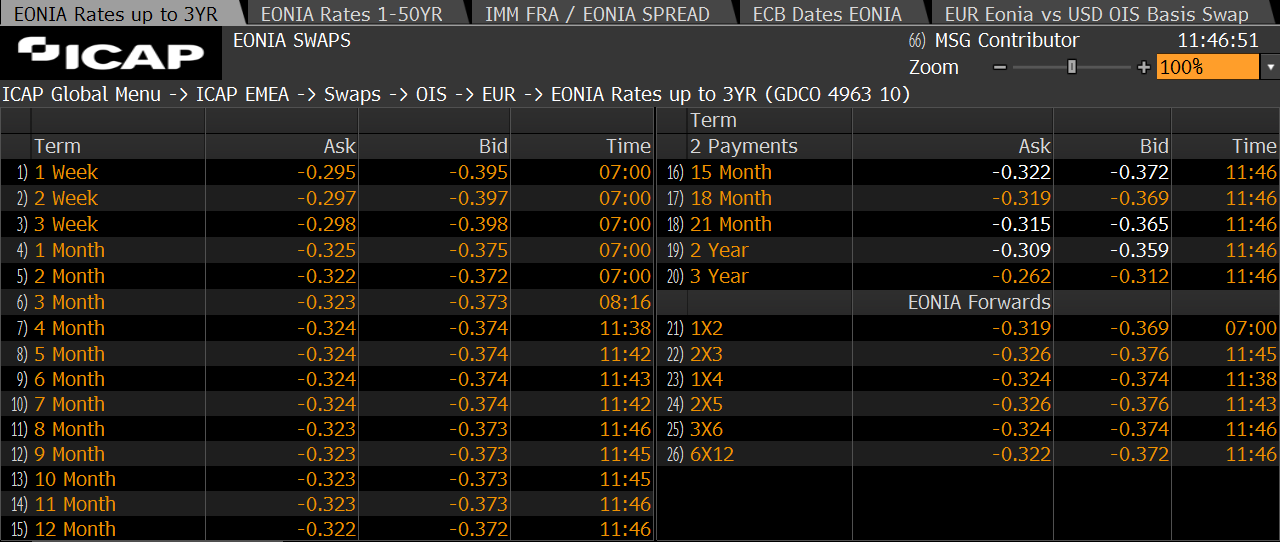
\includegraphics{icap_3.png}

As part of our Quants duties we have set up an Excel spreadsheet which
acquires this data from Bloomberg in realtime. From this spreadsheet,
it's easy to export the data into a Python file - I have done this and
saved the data in a module called \texttt{ois\_data.py}.

We will use a data set extracted in this way, and derive from it the
corresponding discount curve.

    \begin{Verbatim}[commandchars=\\\{\}]
{\color{incolor}In [{\color{incolor}1}]:} \PY{k+kn}{import} \PY{n+nn}{ois\PYZus{}data}
        \PY{n+nb}{print} \PY{p}{(}\PY{n+nb}{type}\PY{p}{(}\PY{n}{ois\PYZus{}data}\PY{o}{.}\PY{n}{quotes}\PY{p}{)}\PY{p}{)}
\end{Verbatim}

    \begin{Verbatim}[commandchars=\\\{\}]
<class 'list'>

    \end{Verbatim}

    \begin{Verbatim}[commandchars=\\\{\}]
{\color{incolor}In [{\color{incolor}2}]:} \PY{n}{ois\PYZus{}data}\PY{o}{.}\PY{n}{quotes}\PY{p}{[}\PY{l+m+mi}{0}\PY{p}{]}
\end{Verbatim}

\begin{Verbatim}[commandchars=\\\{\}]
{\color{outcolor}Out[{\color{outcolor}2}]:} \{'months': 1, 'rate': -0.35\}
\end{Verbatim}
            
    \begin{Verbatim}[commandchars=\\\{\}]
{\color{incolor}In [{\color{incolor}3}]:} \PY{n}{ois\PYZus{}data}\PY{o}{.}\PY{n}{quotes}\PY{p}{[}\PY{o}{\PYZhy{}}\PY{l+m+mi}{1}\PY{p}{]}
\end{Verbatim}

\begin{Verbatim}[commandchars=\\\{\}]
{\color{outcolor}Out[{\color{outcolor}3}]:} \{'months': 720, 'rate': 0.997\}
\end{Verbatim}
            
    \begin{Verbatim}[commandchars=\\\{\}]
{\color{incolor}In [{\color{incolor}4}]:} \PY{n}{ois\PYZus{}data}\PY{o}{.}\PY{n}{observation\PYZus{}date}
\end{Verbatim}

\begin{Verbatim}[commandchars=\\\{\}]
{\color{outcolor}Out[{\color{outcolor}4}]:} datetime.date(2019, 10, 30)
\end{Verbatim}
            
    \hypertarget{building-ois-instances}{%
\subsubsection{Building OIS instances}\label{building-ois-instances}}

We can use the newly created function to build the OIS instances
(\texttt{generate\_swap\_dates}). This function can then be used to
build an OIS object based on the data contained in ois\_data.

    \begin{Verbatim}[commandchars=\\\{\}]
{\color{incolor}In [{\color{incolor}8}]:} \PY{c+c1}{\PYZsh{} first check the 15 months rate}
        \PY{n}{ois\PYZus{}data}\PY{o}{.}\PY{n}{quotes}\PY{p}{[}\PY{l+m+mi}{12}\PY{p}{]}
\end{Verbatim}

\begin{Verbatim}[commandchars=\\\{\}]
{\color{outcolor}Out[{\color{outcolor}8}]:} \{'months': 15, 'rate': -0.35\}
\end{Verbatim}
            
    \begin{Verbatim}[commandchars=\\\{\}]
{\color{incolor}In [{\color{incolor}5}]:} \PY{k+kn}{from} \PY{n+nn}{finmarkets} \PY{k}{import} \PY{n}{OvernightIndexSwap}\PY{p}{,} \PY{n}{generate\PYZus{}swap\PYZus{}dates}
        
        \PY{c+c1}{\PYZsh{} with the new function generates all the dates from the}
        \PY{c+c1}{\PYZsh{} observation up to 15 months }
        \PY{n}{ois} \PY{o}{=} \PY{n}{OvernightIndexSwap}\PY{p}{(}\PY{l+m+mf}{1e6}\PY{p}{,}
                                 \PY{n}{generate\PYZus{}swap\PYZus{}dates}\PY{p}{(}\PY{n}{ois\PYZus{}data}\PY{o}{.}\PY{n}{observation\PYZus{}date}\PY{p}{,} \PY{l+m+mi}{15}\PY{p}{)}\PY{p}{,}                        
                                 \PY{o}{\PYZhy{}}\PY{l+m+mf}{0.35}
                                \PY{p}{)}
        \PY{c+c1}{\PYZsh{} print the last payment date (15 months after obs date)}
        \PY{n}{ois}\PY{o}{.}\PY{n}{payment\PYZus{}dates}\PY{p}{[}\PY{o}{\PYZhy{}}\PY{l+m+mi}{1}\PY{p}{]}
\end{Verbatim}

\begin{Verbatim}[commandchars=\\\{\}]
{\color{outcolor}Out[{\color{outcolor}5}]:} datetime.date(2021, 1, 30)
\end{Verbatim}
            
    \begin{Verbatim}[commandchars=\\\{\}]
{\color{incolor}In [{\color{incolor}7}]:} \PY{c+c1}{\PYZsh{} remember we could use the npv method to }
        \PY{c+c1}{\PYZsh{} calculate the OIS\PYZsq{}s npv}
        \PY{c+c1}{\PYZsh{} only problem is we don\PYZsq{}t yet have a discount }
        \PY{c+c1}{\PYZsh{} curve with which to evaluate it!}
        
        \PY{n}{ois}\PY{o}{.}\PY{n}{npv}\PY{p}{(}\PY{n}{curve}\PY{p}{)}
\end{Verbatim}

    \begin{Verbatim}[commandchars=\\\{\}]

        ---------------------------------------------------------------------------

        NameError                                 Traceback (most recent call last)

        <ipython-input-7-f4413985072e> in <module>()
          4 \# curve with which to evaluate it!
          5 
    ----> 6 ois.npv(curve)
    

        NameError: name 'curve' is not defined

    \end{Verbatim}

    \hypertarget{bootstrapping}{%
\subsubsection{Bootstrapping}\label{bootstrapping}}

In the next we are going to somehow reverse what we did last week where
we determined the OIS's NPV given a certain discount curve.

The general idea here is to find the discount curve such that it prices
correctly each OIS, or at least as well as possible, by minimizing the
sum of the square NPVs:

\[\mathrm{min}_{curve} \Big\{\sum_{i=1}^{n}\mathrm{NPV}(\mathrm{ois}_i, \mathrm{curve})^2\Big\}\]

This description of the problem does not, in theory, specify any
constraints on the pillar dates of the discount curve. However, the
pillar dates determine the number of unknown variables (i.e.~the
dimensionality \(n\) of the optimization problem). A curve with \(n\)
pillar dates has \(n\) pillar discount factors (note that the first
discount factor with value date equal to the today date, is constrained
to 1, so it doesn't count).

In practice, therefore, it makes sense to choose the pillar dates in
such a way that there are exactly the right number of degrees of freedom
in the optimization to match data. So the natural choide is to choose
the pillar dates of the discount curve equal to the set of expiry dates
of the swaps so that in principle we could find a vector of pillar
discount factor that perfectly recover a zero NPV for every swap.

The reason for this is that each market quote will determine exactly one
\emph{free} discount factor which is not already determined by the other
market quotes - this can be seen by considering the mathematical
expression for calculating the fixed leg of the OIS swaps
(\(f_{\mathrm{fix},~i}=N\cdot K\cdot \frac{d_i - d_{i-1}}{360}\)), and
the way that the payment date schedules are constructed. Therefore, once
we've fixed \(\vec{d}\) to be a vector of pillar dates equal to the
expiry dates of the OIS swaps, and we use the notation \(\vec{x}\) to
represent the vector of pillar discount factors, then the problem
becomes:

\[\mathrm{min}_{\vec{x}} \Big\{\sum_{i=1}^{n}\mathrm{NPV}(\mathrm{ois}_i, \mathrm{curve(\vec{d}, \vec{x})})^2\Big\}\]

In practice this is an optmization problem: \textbf{to find the minimum
of the above expression as a function of \(\vec{x}\)}, so we can just
use one the available numerical optimization routines.

So let's start by defining a set of OIS objects to cover all the
maturities defined by the market data we have collected in the
\texttt{ois\_data.py} file.

    \begin{Verbatim}[commandchars=\\\{\}]
{\color{incolor}In [{\color{incolor}10}]:} \PY{k+kn}{from} \PY{n+nn}{finmarkets} \PY{k}{import} \PY{n}{DiscountCurve}\PY{p}{,} \PY{n}{OvernightIndexSwap}\PY{p}{,} \PY{n}{generate\PYZus{}swap\PYZus{}dates}
         \PY{k+kn}{import} \PY{n+nn}{ois\PYZus{}data}
         
         \PY{n}{pillar\PYZus{}dates} \PY{o}{=} \PY{p}{[}\PY{n}{ois\PYZus{}data}\PY{o}{.}\PY{n}{observation\PYZus{}date}\PY{p}{]}
         
         \PY{n}{swaps} \PY{o}{=} \PY{p}{[}\PY{p}{]} \PY{c+c1}{\PYZsh{} container of the OIS objects}
         
         \PY{k}{for} \PY{n}{quote} \PY{o+ow}{in} \PY{n}{ois\PYZus{}data}\PY{o}{.}\PY{n}{quotes}\PY{p}{:}
             \PY{n}{swap} \PY{o}{=} \PY{n}{OvernightIndexSwap}\PY{p}{(}
                 \PY{c+c1}{\PYZsh{} notional \PYZhy{} doesn\PYZsq{}t really matter what we put here}
                 \PY{l+m+mf}{1e6}\PY{p}{,}
                 
                 \PY{c+c1}{\PYZsh{} payment dates}
                 \PY{n}{generate\PYZus{}swap\PYZus{}dates}\PY{p}{(}
                     \PY{n}{ois\PYZus{}data}\PY{o}{.}\PY{n}{observation\PYZus{}date}\PY{p}{,}
                     \PY{n}{quote}\PY{p}{[}\PY{l+s+s1}{\PYZsq{}}\PY{l+s+s1}{months}\PY{l+s+s1}{\PYZsq{}}\PY{p}{]}
                 \PY{p}{)}\PY{p}{,}
                 
                 \PY{c+c1}{\PYZsh{} the fixed rate (in the file is expressed in percent)}
                 \PY{l+m+mf}{0.01} \PY{o}{*} \PY{n}{quote}\PY{p}{[}\PY{l+s+s1}{\PYZsq{}}\PY{l+s+s1}{rate}\PY{l+s+s1}{\PYZsq{}}\PY{p}{]}
             \PY{p}{)}
             \PY{n}{swaps}\PY{o}{.}\PY{n}{append}\PY{p}{(}\PY{n}{swap}\PY{p}{)}
             \PY{n}{pillar\PYZus{}dates}\PY{o}{.}\PY{n}{append}\PY{p}{(}\PY{n}{swap}\PY{o}{.}\PY{n}{payment\PYZus{}dates}\PY{p}{[}\PY{o}{\PYZhy{}}\PY{l+m+mi}{1}\PY{p}{]}\PY{p}{)}
             
         \PY{n}{pillar\PYZus{}dates} \PY{o}{=} \PY{n+nb}{sorted}\PY{p}{(}\PY{n}{pillar\PYZus{}dates}\PY{p}{)}
         \PY{n}{n\PYZus{}df\PYZus{}vector} \PY{o}{=} \PY{n+nb}{len}\PY{p}{(}\PY{n}{pillar\PYZus{}dates}\PY{p}{)}
\end{Verbatim}

    \begin{Verbatim}[commandchars=\\\{\}]
{\color{incolor}In [{\color{incolor}11}]:} \PY{n+nb}{type}\PY{p}{(}\PY{n}{pillar\PYZus{}dates}\PY{p}{)}\PY{p}{,} \PY{n+nb}{len}\PY{p}{(}\PY{n}{pillar\PYZus{}dates}\PY{p}{)}\PY{p}{,} \PY{n}{pillar\PYZus{}dates}\PY{p}{[}\PY{l+m+mi}{0}\PY{p}{]}\PY{p}{,} \PY{n}{pillar\PYZus{}dates}\PY{p}{[}\PY{o}{\PYZhy{}}\PY{l+m+mi}{1}\PY{p}{]}
\end{Verbatim}

\begin{Verbatim}[commandchars=\\\{\}]
{\color{outcolor}Out[{\color{outcolor}11}]:} (list, 34, datetime.date(2019, 10, 30), datetime.date(2079, 10, 30))
\end{Verbatim}
            
    Every optimization algorithm needs an \emph{objective function} i.e.~the
function that is actually minimized to reach our goal. In our case we
want to find the discount curve which minimize the sum of the squared
NPVs (x will be our result aka the list of \emph{best} discount
factors*):

    \begin{Verbatim}[commandchars=\\\{\}]
{\color{incolor}In [{\color{incolor}12}]:} \PY{k}{def} \PY{n+nf}{objective\PYZus{}function}\PY{p}{(}\PY{n}{x}\PY{p}{)}\PY{p}{:}
             
             \PY{n}{curve} \PY{o}{=} \PY{n}{DiscountCurve}\PY{p}{(}       
                 \PY{c+c1}{\PYZsh{} today date}
                 \PY{n}{ois\PYZus{}data}\PY{o}{.}\PY{n}{observation\PYZus{}date}\PY{p}{,}
                 
                 \PY{c+c1}{\PYZsh{} pillar dates}
                 \PY{n}{pillar\PYZus{}dates}\PY{p}{,}
                 
                 \PY{c+c1}{\PYZsh{} pillar discount factors}
                 \PY{n}{x}
             \PY{p}{)}
             
             \PY{n}{sum\PYZus{}sq} \PY{o}{=} \PY{l+m+mf}{0.0}
             
             \PY{k}{for} \PY{n}{swap} \PY{o+ow}{in} \PY{n}{swaps}\PY{p}{:}
                 \PY{n}{sum\PYZus{}sq} \PY{o}{+}\PY{o}{=} \PY{n}{swap}\PY{o}{.}\PY{n}{npv}\PY{p}{(}\PY{n}{curve}\PY{p}{)} \PY{o}{*}\PY{o}{*} \PY{l+m+mi}{2}
                 
             \PY{k}{return} \PY{n}{sum\PYZus{}sq}
\end{Verbatim}

    To optimize our \(\vec{x}\) we can use the \texttt{minimize} algorithm
defined in \texttt{scipy.optimize}.

    \begin{Verbatim}[commandchars=\\\{\}]
{\color{incolor}In [{\color{incolor}13}]:} \PY{k+kn}{from} \PY{n+nn}{scipy}\PY{n+nn}{.}\PY{n+nn}{optimize} \PY{k}{import} \PY{n}{minimize}
         
         \PY{c+c1}{\PYZsh{} initialize to 1 the x vector (random choice)}
         \PY{n}{x0} \PY{o}{=} \PY{p}{[}\PY{l+m+mf}{1.0} \PY{k}{for} \PY{n}{i} \PY{o+ow}{in} \PY{n+nb}{range}\PY{p}{(}\PY{n}{n\PYZus{}df\PYZus{}vector}\PY{p}{)}\PY{p}{]} 
         
         \PY{c+c1}{\PYZsh{} set wide constraints on the discount factors}
         \PY{c+c1}{\PYZsh{} in the minimization problem the value of each x\PYZus{}i}
         \PY{c+c1}{\PYZsh{} will be bound between these limits}
         \PY{n}{bounds} \PY{o}{=} \PY{p}{[}\PY{p}{(}\PY{l+m+mf}{0.01}\PY{p}{,} \PY{l+m+mf}{100.0}\PY{p}{)} \PY{k}{for} \PY{n}{i} \PY{o+ow}{in} \PY{n+nb}{range}\PY{p}{(}\PY{n}{n\PYZus{}df\PYZus{}vector}\PY{p}{)}\PY{p}{]} 
         
         \PY{c+c1}{\PYZsh{} in addition we have an additional constraint:}
         \PY{c+c1}{\PYZsh{} we want the first pillar to be 1 (fixed)}
         \PY{c+c1}{\PYZsh{} (because it has pillar date = today)}
         \PY{n}{bounds}\PY{p}{[}\PY{l+m+mi}{0}\PY{p}{]} \PY{o}{=} \PY{p}{(}\PY{l+m+mf}{1.0}\PY{p}{,} \PY{l+m+mf}{1.0}\PY{p}{)}
         
         \PY{c+c1}{\PYZsh{} finally we run the minimization}
         \PY{n}{result} \PY{o}{=} \PY{n}{minimize}\PY{p}{(}\PY{n}{objective\PYZus{}function}\PY{p}{,} \PY{n}{x0}\PY{p}{,} \PY{n}{bounds}\PY{o}{=}\PY{n}{bounds}\PY{p}{)}
\end{Verbatim}

    \begin{Verbatim}[commandchars=\\\{\}]
{\color{incolor}In [{\color{incolor}14}]:} \PY{c+c1}{\PYZsh{} print the diagnostic of the minimization problem}
         \PY{n}{result}
\end{Verbatim}

\begin{Verbatim}[commandchars=\\\{\}]
{\color{outcolor}Out[{\color{outcolor}14}]:}       fun: 0.000737067806478276
          hess\_inv: <34x34 LbfgsInvHessProduct with dtype=float64>
               jac: array([ 6.40060919e+05, -4.10141278e+01, -1.97120762e+01,  5.02186770e+00,
                 3.16953828e+01,  6.01053281e+01,  9.22468259e+01,  1.25056055e+02,
                 1.61067035e+02,  1.97872773e+02,  2.37837001e+02,  2.78325327e+02,
                -9.76591575e+02, -3.98919050e+02, -3.70947586e+02, -3.33820367e+02,
                -3.09413767e+02,  1.33740400e+02,  5.96171630e+02,  9.90164849e+02,
                 1.18880634e+03,  1.09651231e+03,  7.00761702e+02,  8.12483823e+01,
                -6.55803166e+02, -1.36412700e+03, -1.91306081e+02,  1.92698529e+03,
                 5.34498413e+02, -1.56729815e+02, -5.39276839e+02, -2.47024084e+03,
                -1.83758059e+02,  1.89609719e+03])
           message: b'CONVERGENCE: REL\_REDUCTION\_OF\_F\_<=\_FACTR*EPSMCH'
              nfev: 840
               nit: 12
            status: 0
           success: True
                 x: array([1.        , 1.00030147, 1.00058831, 1.00089012, 1.00118751,
                1.00147996, 1.00178743, 1.00208107, 1.00238467, 1.00267865,
                1.00298261, 1.00327737, 1.00357104, 1.00446948, 1.00531932,
                1.00615237, 1.00694015, 1.00907035, 1.00931983, 1.00710503,
                1.00189947, 0.99379259, 0.98332953, 0.9710012 , 0.95721995,
                0.94267437, 0.92772436, 0.88312793, 0.81780916, 0.7655247 ,
                0.71986347, 0.64350408, 0.5928013 , 0.5454718 ])
\end{Verbatim}
            
    \begin{Verbatim}[commandchars=\\\{\}]
{\color{incolor}In [{\color{incolor}17}]:} \PY{c+c1}{\PYZsh{} objective function value with starting point parameters}
         \PY{n}{objective\PYZus{}function}\PY{p}{(}\PY{n}{x0}\PY{p}{)} 
\end{Verbatim}

\begin{Verbatim}[commandchars=\\\{\}]
{\color{outcolor}Out[{\color{outcolor}17}]:} 1055914177798.2069
\end{Verbatim}
            
    \begin{Verbatim}[commandchars=\\\{\}]
{\color{incolor}In [{\color{incolor}18}]:} \PY{c+c1}{\PYZsh{} objective function value with final values}
         \PY{n}{objective\PYZus{}function}\PY{p}{(}\PY{n}{result}\PY{o}{.}\PY{n}{x}\PY{p}{)} 
\end{Verbatim}

\begin{Verbatim}[commandchars=\\\{\}]
{\color{outcolor}Out[{\color{outcolor}18}]:} 0.000737067806478276
\end{Verbatim}
            
    \begin{Verbatim}[commandchars=\\\{\}]
{\color{incolor}In [{\color{incolor}21}]:} \PY{c+c1}{\PYZsh{} define the discount curve object using the }
         \PY{c+c1}{\PYZsh{} resulting discount factors (result.x)}
         \PY{n}{curve} \PY{o}{=} \PY{n}{DiscountCurve}\PY{p}{(}\PY{n}{ois\PYZus{}data}\PY{o}{.}\PY{n}{observation\PYZus{}date}\PY{p}{,} \PY{n}{pillar\PYZus{}dates}\PY{p}{,} \PY{n}{result}\PY{o}{.}\PY{n}{x}\PY{p}{)}
         
         \PY{k+kn}{from} \PY{n+nn}{datetime} \PY{k}{import} \PY{n}{date}
         \PY{n}{curve}\PY{o}{.}\PY{n}{df}\PY{p}{(}\PY{n}{date}\PY{p}{(}\PY{l+m+mi}{2059}\PY{p}{,} \PY{l+m+mi}{11}\PY{p}{,} \PY{l+m+mi}{23}\PY{p}{)}\PY{p}{)}
\end{Verbatim}

\begin{Verbatim}[commandchars=\\\{\}]
{\color{outcolor}Out[{\color{outcolor}21}]:} 0.643157206728785
\end{Verbatim}
            
    \begin{Verbatim}[commandchars=\\\{\}]
{\color{incolor}In [{\color{incolor}23}]:} \PY{c+c1}{\PYZsh{} 50 years rate }
         \PY{k+kn}{import} \PY{n+nn}{math}
         \PY{o}{\PYZhy{}}\PY{n}{math}\PY{o}{.}\PY{n}{log}\PY{p}{(}\PY{n}{curve}\PY{o}{.}\PY{n}{df}\PY{p}{(}\PY{n}{date}\PY{p}{(}\PY{l+m+mi}{2059}\PY{p}{,} \PY{l+m+mi}{11}\PY{p}{,} \PY{l+m+mi}{23}\PY{p}{)}\PY{p}{)}\PY{p}{)} \PY{o}{/} \PY{l+m+mi}{50}
\end{Verbatim}

\begin{Verbatim}[commandchars=\\\{\}]
{\color{outcolor}Out[{\color{outcolor}23}]:} 0.00882732190315717
\end{Verbatim}
            
    \begin{Verbatim}[commandchars=\\\{\}]
{\color{incolor}In [{\color{incolor}26}]:} \PY{n+nb}{list}\PY{p}{(}\PY{n}{result}\PY{o}{.}\PY{n}{x}\PY{p}{)}
\end{Verbatim}

\begin{Verbatim}[commandchars=\\\{\}]
{\color{outcolor}Out[{\color{outcolor}26}]:} [1.0,
          1.0003014747310168,
          1.000588313127077,
          1.0008901199536386,
          1.0011875146572378,
          1.0014799598670674,
          1.0017874342847497,
          1.0020810669287863,
          1.002384668218312,
          1.0026786511290502,
          1.0029826146845602,
          1.003277367891063,
          1.0035710351042981,
          1.0044694772149225,
          1.0053193209371638,
          1.006152366379903,
          1.0069401522566988,
          1.009070346753292,
          1.0093198286477054,
          1.0071050311457177,
          1.0018994747802303,
          0.9937925927976946,
          0.9833295330059759,
          0.9710012014584769,
          0.9572199541886813,
          0.9426743720454831,
          0.9277243626192413,
          0.8831279292517638,
          0.8178091614623915,
          0.7655246963531933,
          0.719863473051108,
          0.6435040837229044,
          0.592801300550168,
          0.545471799496346]
\end{Verbatim}
            
    \begin{Verbatim}[commandchars=\\\{\}]
{\color{incolor}In [{\color{incolor}27}]:} \PY{n}{pillar\PYZus{}dates}
\end{Verbatim}

\begin{Verbatim}[commandchars=\\\{\}]
{\color{outcolor}Out[{\color{outcolor}27}]:} [datetime.date(2019, 10, 30),
          datetime.date(2019, 11, 30),
          datetime.date(2019, 12, 30),
          datetime.date(2020, 1, 30),
          datetime.date(2020, 2, 29),
          datetime.date(2020, 3, 30),
          datetime.date(2020, 4, 30),
          datetime.date(2020, 5, 30),
          datetime.date(2020, 6, 30),
          datetime.date(2020, 7, 30),
          datetime.date(2020, 8, 30),
          datetime.date(2020, 9, 30),
          datetime.date(2020, 10, 30),
          datetime.date(2021, 1, 30),
          datetime.date(2021, 4, 30),
          datetime.date(2021, 7, 30),
          datetime.date(2021, 10, 30),
          datetime.date(2022, 10, 30),
          datetime.date(2023, 10, 30),
          datetime.date(2024, 10, 30),
          datetime.date(2025, 10, 30),
          datetime.date(2026, 10, 30),
          datetime.date(2027, 10, 30),
          datetime.date(2028, 10, 30),
          datetime.date(2029, 10, 30),
          datetime.date(2030, 10, 30),
          datetime.date(2031, 10, 30),
          datetime.date(2034, 10, 30),
          datetime.date(2039, 10, 30),
          datetime.date(2044, 10, 30),
          datetime.date(2049, 10, 30),
          datetime.date(2059, 10, 30),
          datetime.date(2069, 10, 30),
          datetime.date(2079, 10, 30)]
\end{Verbatim}
            

    % Add a bibliography block to the postdoc
    
    
    
    \end{document}
